\documentclass[twoside]{article}
\setlength{\oddsidemargin}{-0.5 in}
\setlength{\evensidemargin}{1.5 in}
\setlength{\topmargin}{-0.6 in}
\setlength{\textwidth}{5.5 in}
\setlength{\textheight}{8.5 in}
\setlength{\headsep}{0.5 in}
\setlength{\parindent}{0 in}
\setlength{\parskip}{0.07 in}
\setlength{\marginparwidth}{145pt}

%
% ADD PACKAGES here:
% 12

\usepackage{amsmath,
            amsfonts,
            amssymb,
            graphicx,
            mathtools,
            flexisym,
            marginnote,
            hyperref,
            titlesec}

\usepackage[english]{babel}
\usepackage[utf8]{inputenc}
\usepackage[shortlabels]{enumitem}

\graphicspath{ {images/} }

\hypersetup{
    colorlinks=true,
    linkcolor=blue,
    filecolor=magenta,      
    urlcolor=blue,
}

\titlespacing\section{0pt}{12pt plus 4pt minus 2pt}{0pt plus 2pt minus 2pt}
\titlespacing\subsection{0pt}{12pt plus 4pt minus 2pt}{0pt plus 2pt minus 2pt}

%
% The following commands set up the lecnum (lecture number)
% counter and make various numbering schemes work relative
% to the lecture number.
%
\newcounter{lecnum}
\renewcommand{\thepage}{\thelecnum-\arabic{page}}
\renewcommand{\thesection}{\thelecnum.\arabic{section}}
\renewcommand{\theequation}{\thelecnum.\arabic{equation}}
\renewcommand{\thefigure}{\thelecnum.\arabic{figure}}
\renewcommand{\thetable}{\thelecnum.\arabic{table}}

\newcommand{\aosv}{1044414: Advanced Operating Systems and Virtualization}
\newcommand{\wir}{1038137: Web Information Retrieval}
\newcommand{\va}{1052057: Visual Analytics}
\newcommand{\advprog}{1044416: Advanced Programming}
\newcommand{\dchpc}{1044399: Data Centers and High Perf. Computing}

\newcommand{\qu}[1]{\marginnote{\textcolor{cyan}{#1}}}


%
% The following macro is used to generate the header.
%
\newcommand{\lecture}[4]{
   \pagestyle{myheadings}
   \thispagestyle{plain}
   \newpage
   \setcounter{lecnum}{#4}
   \setcounter{page}{1}
   \noindent
   \begin{center}
   \framebox{
      \vbox{\vspace{2mm}
    \hbox to 7.4in { {\bf #1
    \hfill Spring 2018} }
       \vspace{4mm}
       \hbox to 7.4in { {\Large \hfill Lecture #4: #2  \hfill} }
       \vspace{2mm}
       \hbox to 7.4in { {\it Lecturer: #3 \hfill Scribe: Anxhelo Xhebraj,
       Beatrice Bevilacqua} }
      \vspace{2mm}}
   }
   \end{center}
   \markboth{Lecture #4: #2}{Lecture #4: #2}

   \iffalse
   {\bf Note}: {\it LaTeX template courtesy of UC Berkeley EECS dept.}

   {\bf Disclaimer}: {\it These notes have not been subjected to the
   usual scrutiny reserved for formal publications.  They may be distributed
   outside this class only with the permission of the Instructor.}
   \vspace*{4mm}
   \fi
}
%
% Convention for citations is authors' initials followed by the year.
% For example, to cite a paper by Leighton and Maggs you would type
% \cite{LM89}, and to cite a paper by Strassen you would type \cite{S69}.
% (To avoid bibliography problems, for now we redefine the \cite command.)
% Also commands that create a suitable format for the reference list.
\iffalse
\renewcommand{\cite}[1]{[#1]}
\def\beginrefs{\begin{list}%
        {[\arabic{equation}]}{\usecounter{equation}
         \setlength{\leftmargin}{2.0truecm}\setlength{\labelsep}{0.4truecm}%
         \setlength{\labelwidth}{1.6truecm}}}
\def\endrefs{\end{list}}
\def\bibentry#1{\item[\hbox{[#1]}]}
\fi

%Use this command for a figure; it puts a figure in wherever you want it.
%usage: \fig{NUMBER}{SPACE-IN-INCHES}{CAPTION}
\newcommand{\fig}[3]{
            \vspace{#2}
            \begin{center}
            Figure \thelecnum.#1:~#3
            \end{center}
    }
% Use these for theorems, lemmas, proofs, etc.
\newtheorem{theorem}{Theorem}[lecnum]
\newtheorem{lemma}[theorem]{Lemma}
\newtheorem{proposition}[theorem]{Proposition}
\newtheorem{claim}[theorem]{Claim}
\newtheorem{corollary}[theorem]{Corollary}
\newtheorem{definition}[theorem]{Definition}
\newenvironment{proof}{{\bf Proof:}}{\hfill\rule{2mm}{2mm}}

% **** IF YOU WANT TO DEFINE ADDITIONAL MACROS FOR YOURSELF, PUT THEM HERE:

\newcommand\E{\mathbb{E}}

\begin{document}

\nocite{*}

%FILL IN THE RIGHT INFO.
%\lecture{**LECTURE-NUMBER**}{**DATE**}{**LECTURER**}{**SCRIBE**}

\lecture{\aosv}{March 20}{Alessandro Pellegrini}{6}

%\footnotetext{These notes are partially based on those of Nigel Mansell.}

% **** YOUR NOTES GO HERE:

\section{Memory Management}
\label{sec:Memory Management}


As seen in the previous lecture there might be systems providing NUMA
differently from Uniform Memory Access (UMA). Linux handles both cases similarly
since UMA can be seen as a degenerative NUMA system having just one node.

Each node is described by \texttt{struct pglist_data} (typedefined to
\texttt{pg_data_t}) even if the architecture is UMA. All the nodes structs are
linked together forming a linked list called \texttt{pgdat_list}. In the UMA
case only one \texttt{pg_data_t} structure called \texttt{contig_page_data} is
used. From the kernel version 2.6.16 the \texttt{pgdat_list} has been replaced
by a global array called \texttt{node_data[]} and the iteration over it
is done through macros defined in \texttt{include/linux/mm/zone.h}.

Each node is divided into a number of blocks called \textit{zones} which
represent ranges in physical memory. A zone is described by \texttt{struct
zone_struct} typedefined to \texttt{zone_t} namely \texttt{ZONE_DMA,
ZONE_NORMAL, ZONE_HIGHMEM}.

\begin{description}
    \item \texttt{ZONE_DMA (0:16MB) } on x86 32 bit is associated with the first physical 16MB and
is used for Direct Memory Access. This is done to remain compatible with
constrained devices that are not capable to address more then 16MB. In Linux it
is also for disk access (?).
    \item \texttt{ZONE_NORMAL (16MB:896MB) } is the range of memory that is always mapped to
        the kernel's virtual memory.
    \item \texttt{ZONE_HIGHMEM (896MB:End) } is present if there is more
        physical RAM than can be mapped into the kernel address space. Thus it
        is not directly mapped to the kernel's virtual address space, instead it is remapped whenever it is
        needed. In x86 64 bit this zone is not present since the kernel virtual
        address space is not confined to 1GB therefore all physical memory can
        be directly addressed by the kernel virtual space.
\end{description}

\begin{center}
  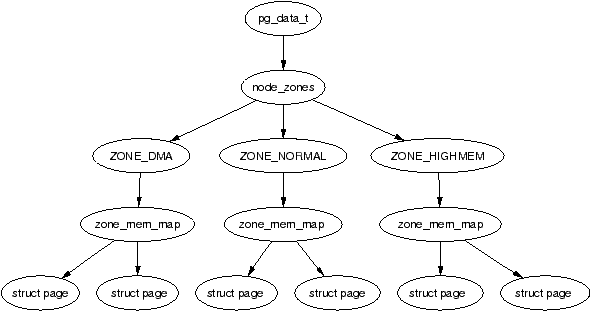
\includegraphics[width=0.8\textwidth]{structrel.png}
  \marginnote{\fig{1}{0 pt}{Relationships between structs. Note that there are multiple
  \texttt{pg_data_t} linked together.}}[-5cm]
\end{center}

To each page frame in the system there is associated a \texttt{struct page}
element that holds all the information needed by the kernel to manage that
frame. All the structs are kept together in a global array called
\texttt{mem_map}.

We are going to describe all the structs represented in Figure 1 starting from
the top of the image.

\marginnote{
    \texttt{pgdat_list} is created incrementally at each
    \texttt{init_bootmem_core} call by prepending each \texttt{pg_data_t}
}[-2cm]


\begin{verbatim}
> include/linux/mmzone.h
typedef struct pglist_data {
    zone_t node_zones[MAX_NR_ZONES];
    zonelist_t node_zonelists[GFP_ZONEMASK+1];
    int nr_zones;
    struct page *node_mem_map;
    unsigned long *valid_addr_bitmap;
    struct bootmem_data *bdata;
    unsigned long node_start_paddr;
    unsigned long node_start_mapnr;
    unsigned long node_size;
    int node_id;
    struct pglist_data *node_next;
} pg_data_t;
\end{verbatim}


\texttt{node_zones[]} holds the \texttt{zone_t} structs for each zone.

\texttt{node_mem_map} is the pointer to the first \texttt{struct page} within
\texttt{mem_map} that belongs to this node (all the other \texttt{struct page}s of the node follow
contiguously in \texttt{mem_map}).

\texttt{node_size} is the total number of page frames belonging to the node.

\texttt{node_next} is the pointer to the next node in the list
\texttt{pgdat_list}.

In the i386 architecture (in which just UMA is supported) the only node
\texttt{contig_page_data} is initialized in \texttt{free_area_init()}
(\texttt{mm/page_alloc.c}) and \texttt{zone_t} fields are filled thanks to the
parameters discovered beforehand through the E820 facility passed to this
function. In the NUMA case (64 bit) node initialization is done in \texttt{setup_arch()} which
indirectly will call \texttt{free_area_init_node()} (\texttt{mm/numa.c}). Both
functions (\texttt{free_area_init_x}) will eventually call
\texttt{free_area_init_core()} (\texttt{mm/page_alloc.c}) that performs the
setup of the data structures described below.

During the POST phase the BIOS discovers how much physical memory is
available and setups a table called E820, which contains information about how
much physical memory is available and which are the usable regions
(for example in case of shadow-ram initialization the BIOS must inform the
kernel that some portion of memory is not available since it stores BIOS
routines).

\newpage

\begin{verbatim}
> include/linux/mmzone.h
typedef struct zone_struct {
    spinlock_t lock;
    unsigned long free_pages;
    zone_watermarks_t watermarks[MAX_NR_ZONES];
    unsigned long need_balance;
    unsigned long nr_active_pages,nr_inactive_pages;
    unsigned long nr_cache_pages;
    free_area_t free_area[MAX_ORDER];
    wait_queue_head_t *wait_table;
    unsigned long wait_table_size;
    unsigned long wait_table_shift;
    struct pglist_data *zone_pgdat;
    struct page *zone_mem_map;
    unsigned long zone_start_paddr;
    unsigned long zone_start_mapnr;
    char *name;
    unsigned long size;
    unsigned long realsize;
} zone_t;
\end{verbatim}

\texttt{lock} is used to protect the zone from concurrent accesses.

\texttt{free_area[]} is an array of structs used for memory allocation by the
Buddy System.

\texttt{zone_mem_map} similarly to \texttt{node_mem_map} points to the first
\texttt{struct page} of \texttt{mem_map} that belongs to this zone.

\begin{verbatim}
> include/linux/mm.h
typedef struct page {
    struct list_head list;
    struct address_space *mapping;
    unsigned long index;
    struct page *next_hash;
    atomic_t count;
    unsigned long flags;
    struct list_head lru;
    struct page **prev_hash;

    #if defined(CONFIG_HIGHMEM) || defined(WANT_PAGE_VIRTUAL)
        void *virtual;
    #endif
} mem_map_t
\end{verbatim}

\texttt{list} is a field used to link this \texttt{struct page} to other
\texttt{struct pages} forming a list of pages satisfying a certain property
(e.g. free pages, dirty pages, locked pages etc.).

\texttt{count} tells the number of processes that are using that page frame (). If
it is 0 then it can be put into the list of free pages (usable).

\texttt{flags} describe the status of the frame. 

\texttt{virtual} is used for pages in the highmem area.
virtual then accepts the virtual address of the page if it is mapped to the
kernel address space.

When pages are initialized in \texttt{free_area_init()} the count field is set
to 0 and \texttt{PG_reserved} bit within the \texttt{flags} field is set to 1
so that no memory allocator except for bootmem (which doesn't rely on these data
structures) can allocate that frame. This is done because the Main Memory
subsystem of the kernel will not use the bootmem allocator anymore in its steady
state but new kinds of allocators and therefore it must ensure that there aren't
conflicts between the two.

Frame un-reserving is performed in \texttt{mem_init()}
(\texttt{arch/i386/mm/init.c}) and it will allow the steady state allocator to
start working.

\section{Buddy System}

Fast algorithm. Suffers of fragmentation. Recursively split and find the best fit for the requested memory. 

There is an array of free\_area\_t where the pointer to the free pages is kept into list head. The integer is used as a smart bitmap. 1 bit for a pair of buddies. Any time that you allocate or free one of the two buddies you invert the buddies. 1 means only one of the two buddies is in use while 0 that either both are available or none. 

The mem alloc starts from higher order to lower to find which buddy is best. 


\section{High Memory}

vmap: long duration mapping for multiple physical pages.

kmap: short duration, needs global sync, all the cores running in kernel mode will see that mapping

kmap atomic: short duration but only this cpu will see that mapping, used in interrupt handlers usually. 

Deallocation: vector of counters for each high memory page. 0 is not mapped, not used by anyone else. 1 just been released. more than 1 it is mapped multiple times. The release is done with kunmap that decrements the counter. When the counter goes to 1 means that no kernel thread is referencing that page.

On mapping we create a PTE.

All the CR3 registers point to the same page table since it is not useful to have different views on memory. When counter 1 the PTE is removed and the tlb is flushed to be sure that all the cores remove that from tlb. 

The struct pages hold the physical addresses of the pages that are then translated to virtual ones.

Memory allocation is finalised with mem init. Destroys the bootmem allocator and releases all the frames used by bootmem through the PG reserved bit. free page is invoked for each page that is freed to give them to buddy. The page count is set to one and free page is called to fake the buddy into thinking that this was actual freed by some kernel subsystem.

The memory allocator is general and doesn't know who is asking for the memory. Process context or Interrupt.

API offered by the buddy system for kernel internal allocation (kernel modules etc.). Get zeroed page, zeros the content and return the virtual address.

Get free pages increases the likelihood of fragmentation.

free page puts back a page into the free list. Failing to pass addr or order might spoil the kernel.


Allocations accept flags. GFP atomic won't put to sleep the asker, used for interrupt context. USER can put to sleep used for userspace. KERNEL is for kernel while BUFFER for buffers to pass data structures to userspace for example. Sleeping the kernel means the thread asking.

In case of NUMA we must also tell which numa node we want to allocate memory etc. or in case of Get free pages returns any numa node etc. Various NUMA policies are specified on how the node is chosen and can be set through set mempolicy. nodemask tell which nodes are involved and maxnode how many bits of the maks need to be checked. The modes can be default which asks for memory from the same node in which the request is issued. bind is from where I was spawned. Interleave different node on each allocation. Preferred you choose.

mbind sets a numa policy for a range of addresses.

move pages is used to move from one numa node to the other. A set of pages moved to a set of nodes and the status tells whether the call succeeded. The cache controllers of the various cores read and communicate for moving pages. 1 line is 64 Bytes therefore there is great overhead to move pages.

Issues are fragmentations (internal and external). Latency. For each numa node there is a buddy system. Anytime asking pages and releasing a spinlock is used.

Fast allocators allow quick allocation through caching. SLAB a block is used. SLUB is the default and is an optimisation of SLAB.

\newpage
\bibliography{Lec6}
\bibliographystyle{plainnat}
\end{document}
